\chapter{Rivelatori per neutroni veloci}
La rivelazione dei neutroni veloci avviene principalmente attraverso la reazione dello scattering elastico, il materiale migliore risulta
l'idrogeno che assorbe la maggior parte dell'energia con il rinculo.
Se le energie sono sopra il keV \`e possibile utilizzare questo meccanisco per eseguire spettroscopia di neutroni.
\section{Conteggio di neutroni veloci}
Per effettuare il solo conteggio di neutroni veloci \`e possibile utilizzare le tecniche dei neutroni lenti moderando prima i neutroni veloci.
Un materiale come il PET o la paraffina ad alto contenuto di idrogeno viene posto attorno al rivelatore (LiI), i neutroni scatterano e rallentano
nel moderatore, successivamente vengono rivelati attraverso la cattura nel rivelatore.
In questi rivelatori \`e fondamentale scegliere il corretto spessore del moderatore: se lo spessore \`e troppo grande allora i neutroni rischiano
di venire assorbiti nel moderatore, se \`e troppo piccolo allora il rischio \`e di avere neutroni troppo energetici che non vengono catturati.
Lo spessore corretto viene determinando per quale spessore si osserva il massimo del tasso di conteggi.
\begin{figure}[htbp]
\begin{center}
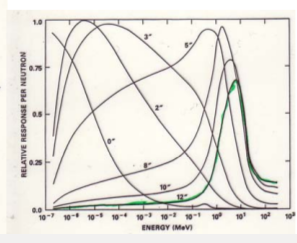
\includegraphics[scale=1]{./Immagini/Moderatori.png}
\caption{Andamento della funzione di risposta dei rivelatori al variare dello spessore dei rivelatori}
\label{fig:moderatori}
\end{center}
\end{figure}
\subsection{Il dosimetro sferico}
Una geometria molto usata \`e quella sferica.
Sperimentalmente si \`e visto che utilizzando uno spessore di PET di 12 pollici, la funzione di risposta del dispositivo in base all'energia dei neutroni aveva una buona somiglianza
alla dose equivalente rilasciata da neutroni in un tessuto biologico.
Questa coincidenza \`e stata utilizzata per produrre dosimetri sferici per la misura delle dosi assorbite in quanto il numero di neutroni \`e correlabile
alla dose assorbita avendo i giusti fattori di peso ad ogni energia.
\begin{figure}[htbp]
\begin{center}
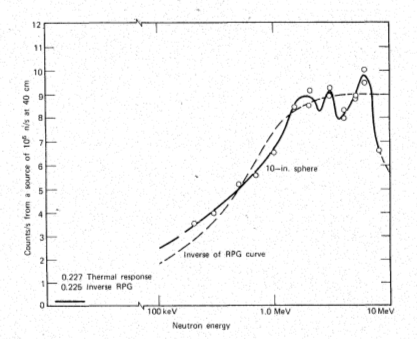
\includegraphics[scale=1]{./Immagini/DoseNeutroni.png}
\caption{Paragone tra dose assorbita e probabilit\`a di assorbimento di un neutrone}
\label{fig:doseNeutroni}
\end{center}
\end{figure}
In questi dosimetri la discriminazione dal fondo $\gamma$ \`e anche facile da effettuare: il Q-valore della reazione \`e elevato, quindi, anche in presenza
di fondi $\gamma$ abbastanza intensi, non si hanno problemi.
\subsection{Contatori a risposta piatta}
Un rivelatore a risposta piatta \`e un rivelatore dove l'efficienza non dipende dall'energia.
\subsubsection{Il contatore lungo}
Un possibile rivelatore a risposta piatta \`e il contatore lungo.
\begin{figure}[htbp]
\begin{center}
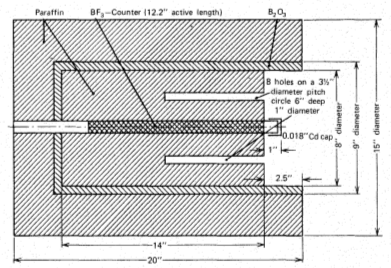
\includegraphics[scale=1]{./Immagini/ContatoreLungo.png}
\caption{Disegno di un contatore lungo}
\label{fig:contatoreLungo}
\end{center}
\end{figure}
Questo rivelatore \`e a geometria cilindrica: i neutroni devono incidere su di esso dalla faccia a destra nella figura~\ref{fig:contatoreLungo}, mentre
gli altri vengono bloccati dal moderatore.
Il rivelatore \`e formato da un rivelatore a BF$_3$ di forma cilindrica posto al centro di un moderatore;
parallelamente al tubo rivelatore sono presenti dei fori per permettere una diversa penetrazione all'interno del rivelatore ai neutroni.
In questo modo \`e possibile rivelare sia neutroni veloci che lenti, i primi potranno essere rivelati se percorreranno molta paraffina,
i secondi se incideranno il rivelatore sulla faccia frontale oppure penetrando nei fori.
Grazie al BF$_3$ il rivelatore permette di distinguere bene i $\gamma$, tuttavia possiede il problema dell'efficienza, essa vale infatti circa
lo 0.25\%.
Per ridurre questo problema \`e possibile sacrificare la capacit\`a di discriminare $\gamma$ utilizzando tubi a $^3$He, portando l'efficienza
al 11.5\%.
\subsubsection{Alternative}
Altre alternative provengono da scintillatori NaI in una sfera di moderatore, oppure scintillatori liquidi o plastici con contenuto di H.
Questi scintillatori rivelano il $\gamma$ prodotto dalla cattura del neutrone da parte dell'idrogeno contenuto nel moderatore (2.2 MeV),
per questo motivo la loro risposta \`e piatta.
\section{Rivelatori basati su reazioni indotte da neutroni veloci}
Una possibile tecnica di spettroscopia pu\`o essere basata sull'utilizzo delle reazioni attivate direttamente dai neutroni veloci.
Tralasciando la diffusione elastica, la cattura di neutroni veloci pu\`o dare informazioni sull'energia, infatti se un neutrone
di energia $E$ viene catturato, verr\`a liberata un energia di $Q+E$;
ad esempio, la cattura del litio-6 ha un Q-valore di 4.78 MeV, per cui neutroni nell'ordine del 100 keV possono essere rivelati
e misurati in energia sottraendo all'energia misurata il Q-valore.
Queste reazioni hanno il problema di avere una sezione d'urto piccolissima, per cui si hanno efficienze molto ridotte.\\
Le reazioni principalmente utilizzate sono quelle del litio-6 e dell'elio-3.
\subsection{Reazioni e rivelatori del litio-6}
La sezione d'urto del litio-6 ha una risonanza a 250 keV, inoltre se il neutrone \`e troppo energetico (sopra i 2.5 MeV) si presenta un 
processo endotermico concorrente che domina, $^6$Li(n,n'd)$^4$He (Q-v=-1.4 MeV), dove viene liberato un neutrone.
Per questo motivo lo spettro atteso dal litio \`e formato da un picco a $Q+E$ dovuto ai neutroni, un continuo dovuto al processo concorrente (il decadimento
\`e a tre corpi), \`e un picco a $Q$ dovuto a neutroni termici che sono sempre presenti nell'ambiente.\\
Un rivelatore basato sul litio \`e uno scintillatore a LiI, esso ha per\`o problemi di non linearit\`a per particelle $\alpha$ e H a temperatura ambiente
per cui la sua FWHM \`e del 40\%.
Si possono ottenere miglioramenti utilizzando il rivelatore a temperature basse, ad esempio con l'azoto liquido si pu\`o portare il rivelatore
ad avere una FWHM del 20\%.\\
Un altro tipo di rivelatore \`e quello basato sui vetri al litio, per via della sua elevata risoluzione temporale, viene utilizzato per effettuare
T.O.F. di fasci di neutroni. 
La scintillazione prodotta dal vetro \`e, tuttavia, piuttosto ridotta, infatti il vetro ha un quenching factor del 25\% per le particelle
prodotte dal decadimento, rendendo difficile la discriminazione dal fondo $\gamma$ (4 MeV vengono visti come un $\gamma$ da un 1 MeV).\\
Un altra possibilit\`a \`e data da fibre scintillanti al litio, poich\`e le $\alpha$ hanno un range di 7 $\mu$m, l'idrogeno di 40 $\mu$m e gli elettroni
di 1 mm, utilizzando fibre del diametro di 100 $\mu$m si pu\`o ottenere una facile discriminazione dal fondo gamma.\\
Utilizzando un sandwich di rivelatori al silicio con in mezzo litio, si pu\`o costruire un rivelatore basato sulla misura della doppia coincidenza.
Se il neutrone non \`e troppo veloce l'approssimazione di radiazione b2b \`e ancora valida e si osservano coincidenze;
se l'energia cresce, tuttavia, le coincidenze iniziano a mancare in quanto la radiazione sar\`a pi\`u proiettata in direzione di un rivelatore.
\subsection{Reazioni e rivelatori con l'elio-3}
Le reazioni predominanti dell'elio fino a 10 MeV sono quelle di cattura e scattering elastico; in particolare la prima cala con l'energia, mentre
la seconda domina sopra i 100 keV.
Lo spettro atteso \`e quindi formato da un picco a $E+Q$, un picco a $Q$ per i neutroni termici, un continuo dovuto allo scattering elastico
con massimo a 0.75$E_n$ (massima energia cedibile all'elio-3), un continuo dovuto ad effetto parete ed impulsi spuri.\\
Un rivelatore utilizzabile nella spettroscopia con l'elio \`e la camera proporzionale.
L'elio che viene utilizzato viene sottoposto ad alta pressione e viene aggiunto del Kr per ridurre l'effetto parete.
Il grande vantaggio di questi rivelatori sta nella possibilit\`a di poter effettuare del PSD.
Quando un nucleo di elio rincula, esso dissipa rapidamente e in un range molto ristretto la propria energia, per questo motivo
gli elettroni prodotti verranno moltiplicati e arriveranno all'anodo in tempi molto simili, generando impulsi veloci.
Allo stesso modo si pu\`o dedurre che impulsi distorti dall'effetto parete avranno rise time molto alti.
Questa distinzione permette di scartare gli impulsi non di interesse (scartando purtroppo anche qualche evento dovuto ai protoni da cattura, circa il 50\%).
Con questa tecnica \`e anche possibile scartare e discriminare gli eventi dovuti a $\gamma$.\\
Un'alternativa \`e la camera a ionizzazione, dove \`e possibile raggiungere un'ottima risoluzione energetica, 20 keV su 1 MeV, a costo di tempi pi\`u lenti.\\
Mescolando l'elio con una piccola frazione nel \% di xenon \`e possibile costruire scintillatori con una buona resa in luce, ottimi per applicazioni
temporali, ma pessime per applicazioni energetiche.\\
\`E possibile impiegare l'elio per uno spettrometro a sandwich, ottenendo efficienze migliori per via della sezione d'urto maggiore;
il problema principale sta nel Q-valore basso che rende difficile la distinzione dal fondo $\gamma$.
\section{Spettroscopia attraverso la diffusione di neutroni}
Per le alte energie \`e possibile effettuare la spettroscopia mediante la reazione di scattering elastico di neutroni sui nuclei.
Per utilizzare questa reazione \`e necessario che i nuclei siano a riposo e di massa comparabile a quella del neutrone, per quanto
riguarda la discriminazione, le tecniche di RTD permettono di distinguere abbastanza bene il fondo $\gamma$.
I neutroni termici sono trascurabili, a parte per la reazione di cattura.
L'energia di diffusione di un nucleo risulta:
\begin{equation*}
E_r=\frac{4A}{(1+A)^2}\, \text{cos}^2\theta E_n
\end{equation*}
in particolare per nuclei che rinculano a $\pi$/2 essa vale 0, per collisioni head-on vale:
\begin{equation*}
E_r=\frac{4A}{(1+A)^2}E_n
\end{equation*}
in particolare per diffusioni contro protoni vale esattamente $E_n$.\\
La probabilit\`a di diffusione a basse energie (sotto i 10 MeV) \`e uniforme per tutti gli angoli e per l'idrogeno vale:
\begin{equation*}
P(E_r)=\frac{1}{E_n}
\end{equation*}
per cui l'energia media di diffusione risulta $E_n/2$.\\
L'efficienza dei rivelatori pu\`o essere calcolata come:
\begin{equation*}
\epsilon= 1 - e^{-N\,\sigma_s\,x} = 1 - e^{-\Sigma_s \, x}
\end{equation*}
mentre empiricamente per il range tra 0.3 e 3 MeV vale la formula empirica:
\begin{equation*}
\sigma_s^{H} = \frac{4.83}{\sqrt{E}} - 0.578 \, \text{barn}
\end{equation*}
\section{Scintillatori per rinculo di protoni}
Utilizzando lo scattering elastico \`e possibile realizzare scintillatori basati sul rinculo di protoni.
Dato che i protoni sono particelle pesanti possiedono un range ridotto, permettendo un completo assorbimento della loro energia;
inoltre questi scintillatori possono essere di qualsiasi tipo, organici, inorganici, liquidi.
L'unico compromesso che \`e necessario trovare \`e quello tra efficienza e FWHM:
la prima aumenta con il volume (e cala con l'energia), mentre la seconda peggiora con il volume, a causa di raccolte peggiori della luce,
aumenti del fondo $\gamma$ (pile-up) e scattering multipli che distorcono la funzione di risposta.
\subsection{Effetti che distorcono lo spettro}
Alcuni effetti possono distorcere lo spettro:
\begin{itemize}
\item La \textbf{risposta dello scintillatore non \`e lineare}, infatti:
\begin{equation*}
H = k \, E^{3/2} \;\;\; \Rightarrow E = k' \, H^{2/3}
\end{equation*}
per cui si ha che lo spettro differenziale invece di essere costante risulta:
\begin{equation*}
\frac{dN}{dE}=\frac{dN}{dH}\frac{dH}{dE} = \alpha \, H^{-1/3}
\end{equation*}
\item Posso avere \textbf{fughe} di protoni che spostano verso il basso l'energia
\item Posso avere \textbf{scattering multipli} che causano una maggior deposizione di energia e uno spostamento verso l'alto dello spettro
\item Posso avere \textbf{scattering su C} che sottrae energia al neutrone (fino al 28\%)
Poich\`e il carbonio ha una resa in luce inferiore l'evento non viene visto, tuttavia se il neutrone scattera contro un protone allora si osserva
una misura distorta in energia
\item Anche con questi effetti mi aspetterei di avere un'energia massima con un \textit{cut-off} brusco; questo non accade per via della \textbf{risoluzione}
dello scintillatore che ammorbidisce il gradino
\item Ad alte energie ho \textbf{reazioni endotermiche del carbonio} in competizione; poich\`e esse emettono particelle cariche pesanti non producono molta luce,
quindi non sono eccessivamente fastidiose
\end{itemize}
\begin{figure}[htbp]
\begin{center}
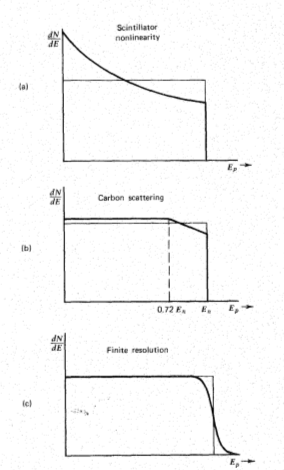
\includegraphics[scale=0.75]{./Immagini/DistorsioniNeutroni.png}
\caption{Alcune distorsioni dello spettro}
\label{fig:distorsioniNeutroni}
\end{center}
\end{figure}
\subsection{Efficienza contro soglia di bias}
In ogni scintillatore \`e necessario imporre delle soglie di discriminazione per fare in modo di evitare di contaminare lo spettro
con impulsi spuri e rumore.
Dato che nella spettroscopia per rinculo lo spettro parte da energia nulla, imporre soglie di bias elimina inevitabilmente parte utile dello spettro;
per questo motivo \`e necessario trovare un compromesso tra soglia di bias ed efficienza.
L'efficienza a soglia nulla viene detta \textbf{efficienza a zero bias}, in generale a parit\`a di soglia l'efficienza cala per energie pi\`u basse.
\subsection{Calibrazione con raggi $\gamma$}
La calibrazione con raggi $\gamma$ pu\`o essere effettuata tenendo bene a mente che la resa in luce degli elettroni \`e maggiore di quella delle
particelle cariche pesanti, per questo si parla di MeVee, ovvero MeV Electron Equivalent.
Per questo motivo una volta effettuata la calibrazione con i fotoni \`e necessario passare dal fattore di quenching per estenderla alle altre particelle.
Dato che si utilizzando rivelatori organici i nuclei sono a basso Z, per cui la sezione d'urto dell'effetto fotoelettrico non \`e molto elevata:
in pratica domina l'effetto Compton, per cui la calibrazione pu\`o essere effettuata unicamente utilizzando la spalla Compton.
Per via della scarsa risoluzione dello scintillatore, individuare questa spalla pu\`o essere molto complicato, per questo la calibrazione \`e molto delicata.
\subsection{Uso del PSD per distinguere i $\gamma$}
Gli impulsi generati da $\gamma$ hanno un fronte di salita molto pi\`u veloce di quelli generati da protoni, per questo motivo \`e possibile effettuare
con buona efficacia la PSD per discriminare i $\gamma$ in arrivo sul rivelatore.
Questo permette di effettuare una spettroscopia $\gamma$ in parallelo a quella dei neutroni;
una volta misurato lo spettro sar\`a, tuttavia, necessario ricorrere a tecniche di deconvoluzione in quanto sono assenti i fotopicchi, poich\`e lo Z \`e basso.
\subsection{Contatori proporzionali}
\`E possibile realizzare contatori proporzionali utilizzando dei gas come H, CH$^4$ o He.
Questi dispositivi hanno un'efficienza piuttosto ridotta (nel 1\%), sono pi\`u difficili da maneggiare e gestire (sono gassosi e ad esempio l'idrogeno \`e esplosivo)
e sono soggetti all'effetto parete, tuttavia hanno una probabilit\`a di scattering multiplo piuttosto ridotta e la discriminazione dai $\gamma$ risulta pi\`u semplice.
La discriminazione del fondo $\gamma$ pu\`o essere effettuata studiando le ampiezza (gli elettroni depositano meno energia e tendono a fuggire)
e effettuando del RTD, in quanto i nuclei rinculanti depositano tutta l'energia localmente, generando impulsi veloci.\\
La scelta dei gas ha diverse conseguenze:
\begin{itemize}
\item utilizzare l'idrogeno \`e ottimo per misurare tutta l'energia, tuttavia ha problemi legati al fatto che va usato a bassa densit\`a per cui ha uno scarso potere frenante
\item utilizzare il metano da problemi legati allo scattering su carbonio, che pu\`o sottrarre fino al 28\% dell'energia)
\item utilizzare l'elio da luogo ad uno spettro non a box, in quanto la sezione d'urto differenziale non \`e isotropa
\end{itemize}
La geometria tipicamente utilizzata \`e quella cilindrica, le disuniformit\`a del campo in prossimit\`a dell'anodo possono generare problemi nello spettro
e posso avere fughe di protoni. 
Quest'ultimo problema pu\`o essere risolto introducendo un catodo a griglia con contatori esterni: quando un protone viene rilevato come in fuga
viene prodotto un impulso collegato ad un modulo di anticoincidenza.
In questo modo gli impulsi parziali per effetto parete possono essere scartati.\\
La calibrazione di questi dispositivi non pu\`o essere effettuata mediante $\gamma$, in quanto gli elettroni non depositano energia.
Per questo motivo si pu\`o introdurre del elio-3 per farlo reagire con i neutroni termici ed effettuare la calibrazione con il Q-valore, tuttavia
questa tecnica ha dei problemi legati al fatto che una delle particelle prodotte non \`e un protone.
L'alternativa \`e l'introduzione di $^{37}$Ar che emette raggi X a 2.82 keV, ma che non \`e ottima in quanto lavora con elettroni.\\
La risposta del rivelatore \`e lineare per rinculi sopra i 10 keV, sotto questa energia si presentano delle non linearit\`a.
\subsection{Telescopi per rinculo di protoni}
In un telescopio per rinculo l'energia del neutrone viene misurata studiando l'energia e l'angolo di diffusione dei protoni.
Per farlo i neutroni vengono collimati su un diffusore ricco di idrogeno; un rivelatore misura l'energia dei protoni diffusi ad un determinato angolo
e invertendo la relazione
\begin{equation*}
E_p = E_n \, \text{cos}^2\theta
\end{equation*}
viene ricavata l'energia del neutrone incidente.
Questa tecnica possiede una serie di problematiche:
\begin{itemize}
\item poich\`e i protoni disperdono facilmente molta energia, \`e necessario che il bersaglio sia sottile (si usano film)
\item il dispositivo deve funzionare in condizioni di vuoto
\item devo stare attento a distinguere il fondo dai protoni, per questo motivo vengono usati solitamente due rivelatori in cascata e si lavora
sulle doppie coincidenze.
Il primo misura una frazione di energia, il secondo la rimanente; dalla frazione depositata nel primo rivelatore, attraverso la formula di Bethe-Bloch, \`e
possibile determinare il tipo di particella che ha depositato l'energia, distinguendo protoni da, per esempio, particelle $\alpha$.
\end{itemize}
L'efficienza di questi dispositivi \`e bassissima, nell'ordine del $10^{-5}$, tuttavia ha il vantaggio di essere calcolabile, in quanto sono note
le sezioni d'urto; essa pu\`o essere migliorata aumentando lo spessore del film e utilizzandolo come rivelatore (ad esempio a scintillazione) per
spettroscopia.
In questo modo si recupera l'informazione sull'energia persa dal protone nel diffusore.
\subsection{Spettromento con gate da cattura}
Supponiamo di costruire uno scintillatore organico grande: quando un neutrone incider\`a su di esso, avverranno una serie di scattering di moderazione
ed infine una cattura. 
Gli scattering avvengono nel tempo di 100 ns, dando luogo ad un unico impulso di scintillazione, mentre la cattura avviene dopo circa 10 $\mu$s.
Per questo motivo si pu\`o pensare di misurare la scintillazione per ottenere l'energia del neutrone incidente, distinguendo l'evento dal
fondo mediante un gate sull'energia di cattura.
La cattura dell'idrogeno risulta insidiosa, in quanto libera $\gamma$ che, nella maggior parte dei casi, fuggono; per questo motivo si arricchisce
lo scintillatore con boro-10, che libera particelle cariche pesanti. 
La valutazione delle coincidenze casuali pu\`o essere fatta senza troppi problemi, purch\`e non siano troppe; in caso di alti rate, questo
non pu\`o essere fatto in quanto le coincidenze sommergono gli eventi reali.\\
L'efficienza di questo tipo di rivelatori \`e nell'ordine del 10\% per neutroni da 1 MeV, fino a 1\% per neutroni da 14 MeV, ma ha il problema
della risoluzione energetica (\`e uno scintillatore) e dello scattering inelastico sul carbonio per energie oltre i 5-6 MeV.\\
Rivelatori alternativi sono liquidi con boro o una combinazione di plastici e vetro con litio-6.
Questi dispositivi permettono di fare PSD per distinguere i $\gamma$ nel primo o per distinguere impulsi da scattering da impulsi da cattura nel secondo.